%!TEX root = ../template.tex
%%%%%%%%%%%%%%%%%%%%%%%%%%%%%%%%%%%%%%%%%%%%%%%%%%%%%%%%%%%%%%%%%%%%
%% chapter2.tex
%% NOVA thesis document file
%%
%% Chapter with the template manual
%%%%%%%%%%%%%%%%%%%%%%%%%%%%%%%%%%%%%%%%%%%%%%%%%%%%%%%%%%%%%%%%%%%%
\chapter{Problem Details}
\label{cha:problem}

This chapter presents in detail the problem faced in this dissertation. It starts by providing the reader with an overview of the agricultural scene, field organisation, the default method for data collection, main economically harmful pests, plants and environmental variables. In the end, it is explained the possibility of full-automation for the biological analysis but the main focus is pseudo-automated data collection: the user has to read the biological variables and register them in an easy and straightforward way.

\section{Agricultural Domain} % (fold)
\label{sec:agricultural_domain}

Agriculture is split into two main groups: Indoor and outdoor. Outdoor is the default; an open air field used to grow plants and trees. Indoor is the more recent approach where an ideal ecosystem is created for the development of plants(usually low species).

Indoor agriculture presents a better opportunity for precision agriculture since the whole growing process is digitally controlled: raditation, water, fertilizer, temperature etc. Vertical Agriculture is growing fast since it provides the best ratio of plants per squared meter. Vertically alligned trays covered in fertile soil can incorporate sensors directly in their design, Internet connectivity is not a problem, rotation of trays can be used for a single multispectral analysis machine to register the growth of all plants, etc. 

\begin{figure}[htbp]
  \centering
  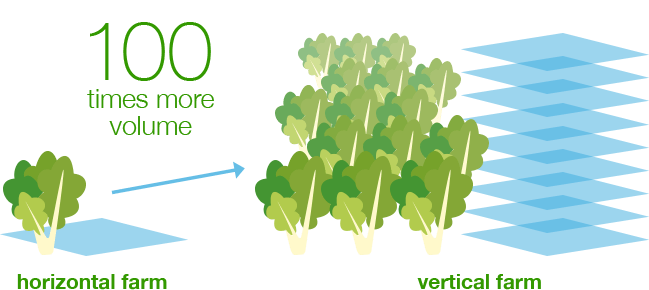
\includegraphics[width=0.7\linewidth]{hor_ver_farming}
  \caption{Vertical farming increases the volume of production per squared meter.}
  \label{fig:horizontal_vertical_farming}
\end{figure}

With these many points in favour, Indoor Vertical Farming is still not the most common farming methodology. Mostly due to the initial costs and evolving/unstable technology, farmers opt by growing their fields the traditional way. This does not mean that farmers fear technology but progress is slow, especially within the more traditional and manual labour communities. 

A farm is a place where agricultural activities take place. For organisational purposes, farms are usually split into plots which provide the first level of organisation.

\begin{figure}[htbp]
  \centering
  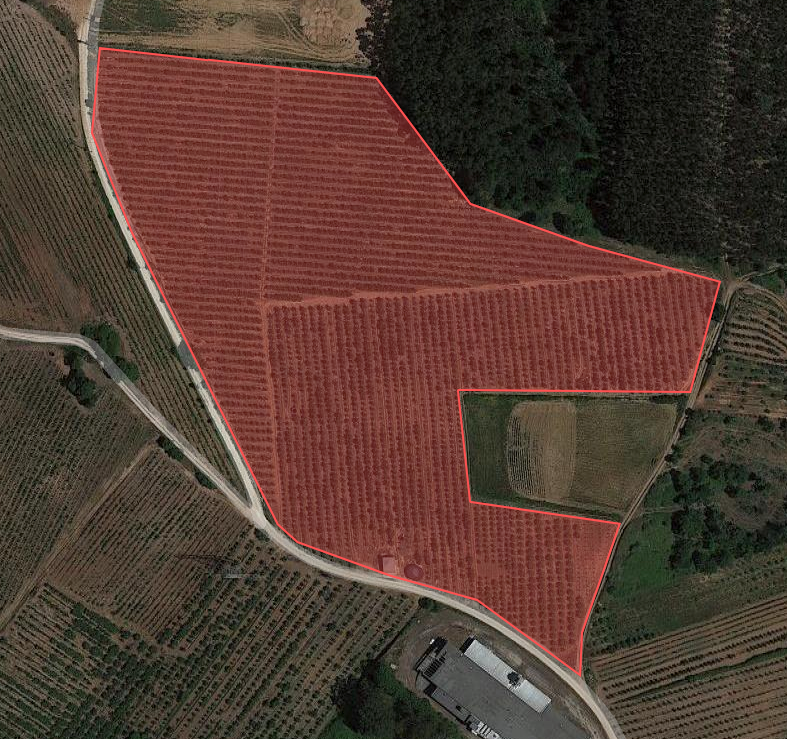
\includegraphics[width=0.5\linewidth]{field_with_plots}
  \caption{Vale Pragrança: a farming field from the FitoAgro project. Three plots are visible in the satellite image.}
  \label{fig:field_with_plots}
\end{figure}

For a plot, a single type of plant is installed. During this dissertation, the focus will be on Royal Gala Apple (Malus pumila) and Pear "Rocha" (Pyrus communis) crops.

\begin{figure}[htbp]
  \centering
  \subcaptionbox{\textit{Malus "Royal Gala"}\label{fig:royal_gala}}%
    {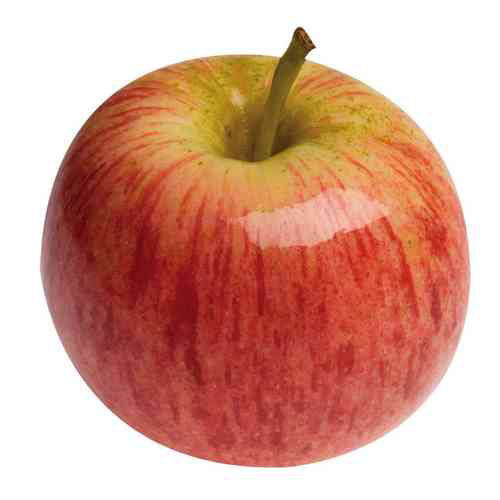
\includegraphics[width=0.5\linewidth]{royal_gala}}%
  \hfill  
  \subcaptionbox{\textit{Pyrus Communis "Rocha"}\label{fig:pear_rocha}}%
    {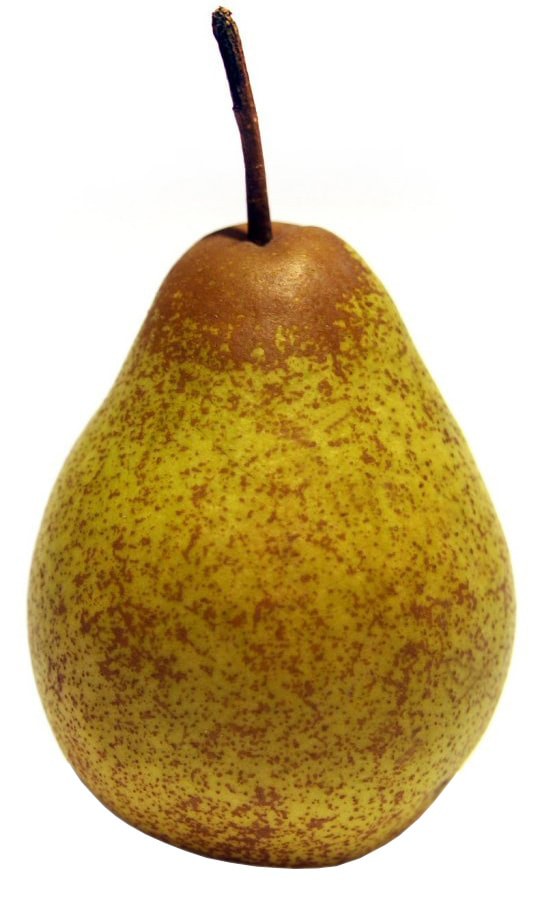
\includegraphics[width=0.4\linewidth]{pera_rocha}}%
  \caption{Crops to be monitored during this dissertation}
  \label{fig:crops_studied}
\end{figure}

\section{Spreadsheets} %%%%%%%%%%%%%%%%%%%%%%%%%%%%%%%%
\label{sec:problem_spreadsheets}

Integrated production by farmers requires certain obligations and responsibilities. Some countries have strict regulation on agriculture while others provide no guidelines for cooperation on agricultural activity. Portugal provides on the DGADR ("Direção-Geral de Agricultura e Desenvolvimento Rural") website a field notebook template for the most common plant cultures grown in Portugal.

These notebooks track the most important things happening during the production cycle: 

\begin{enumerate}
	\item Phenological Growth Stages of the crop
	\item Observations regarding the main enemies of the crop
	\item Dates of the treatments performed on the field and the phytopharmaceutical products used
	\item Production system data (pruning, watering, fertilising and harvesting)
\end{enumerate}

Field notebooks were once used on paper, but nowadays, since teams take turns working on the fields, most agronomists and farmers upload their paper records to online collaborative spreadsheets. 

\subsection{Phenological Growth Stages}
\label{sec:problem_spreadsheets_phenological}

Phenology is the study of periodic plant and animal life cycle events and how these are influenced by seasonal and interannual variations in climate. In the context of this dissertation: the growth rate of a plant and how it is influenced by temperature, light and humidity. 

Precise tracking of the phenological stage of a plant is of the utmost importance since some pests, diseases and products may depend on the current stage.

Different plant species have different phenological stages. Since this work focuses on Pome tree species, namely Apple (Malus Pumila) and Pear (Pyrus Communis) trees, the respective phenological stages of growth are illustrated on \ref{fig:pheno_apple_raw} and \ref{fig:pheno_pear_raw}.

\begin{figure}[htbp]
  \centering
  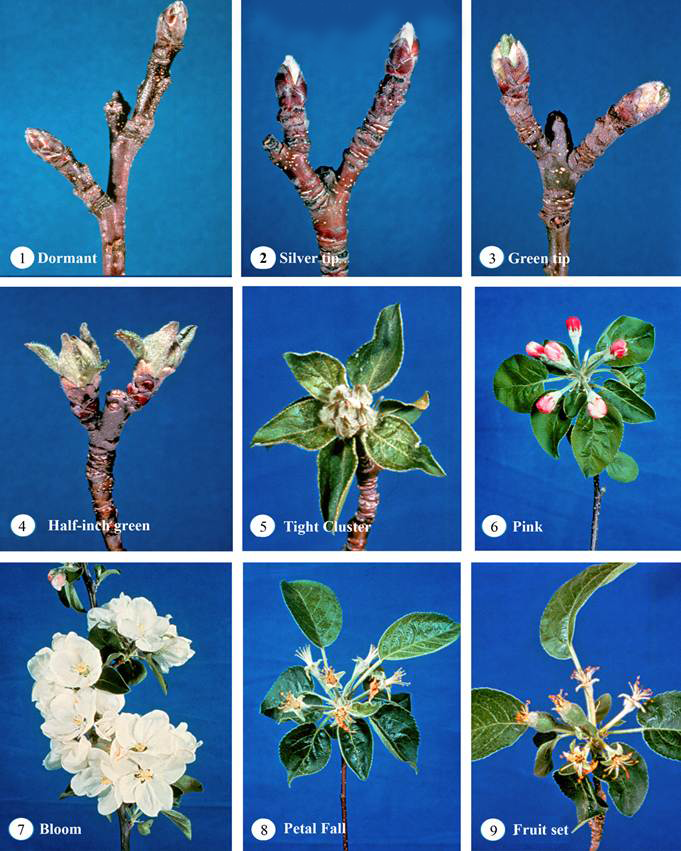
\includegraphics[width=0.7\linewidth]{pheno_apple_raw}
  \caption{Phenological Stages of Malus Pumila - by TheJentschLab \cite{TheJentschLab}}
  \label{fig:pheno_apple_raw}
\end{figure}

\begin{figure}[htbp]
  \centering
  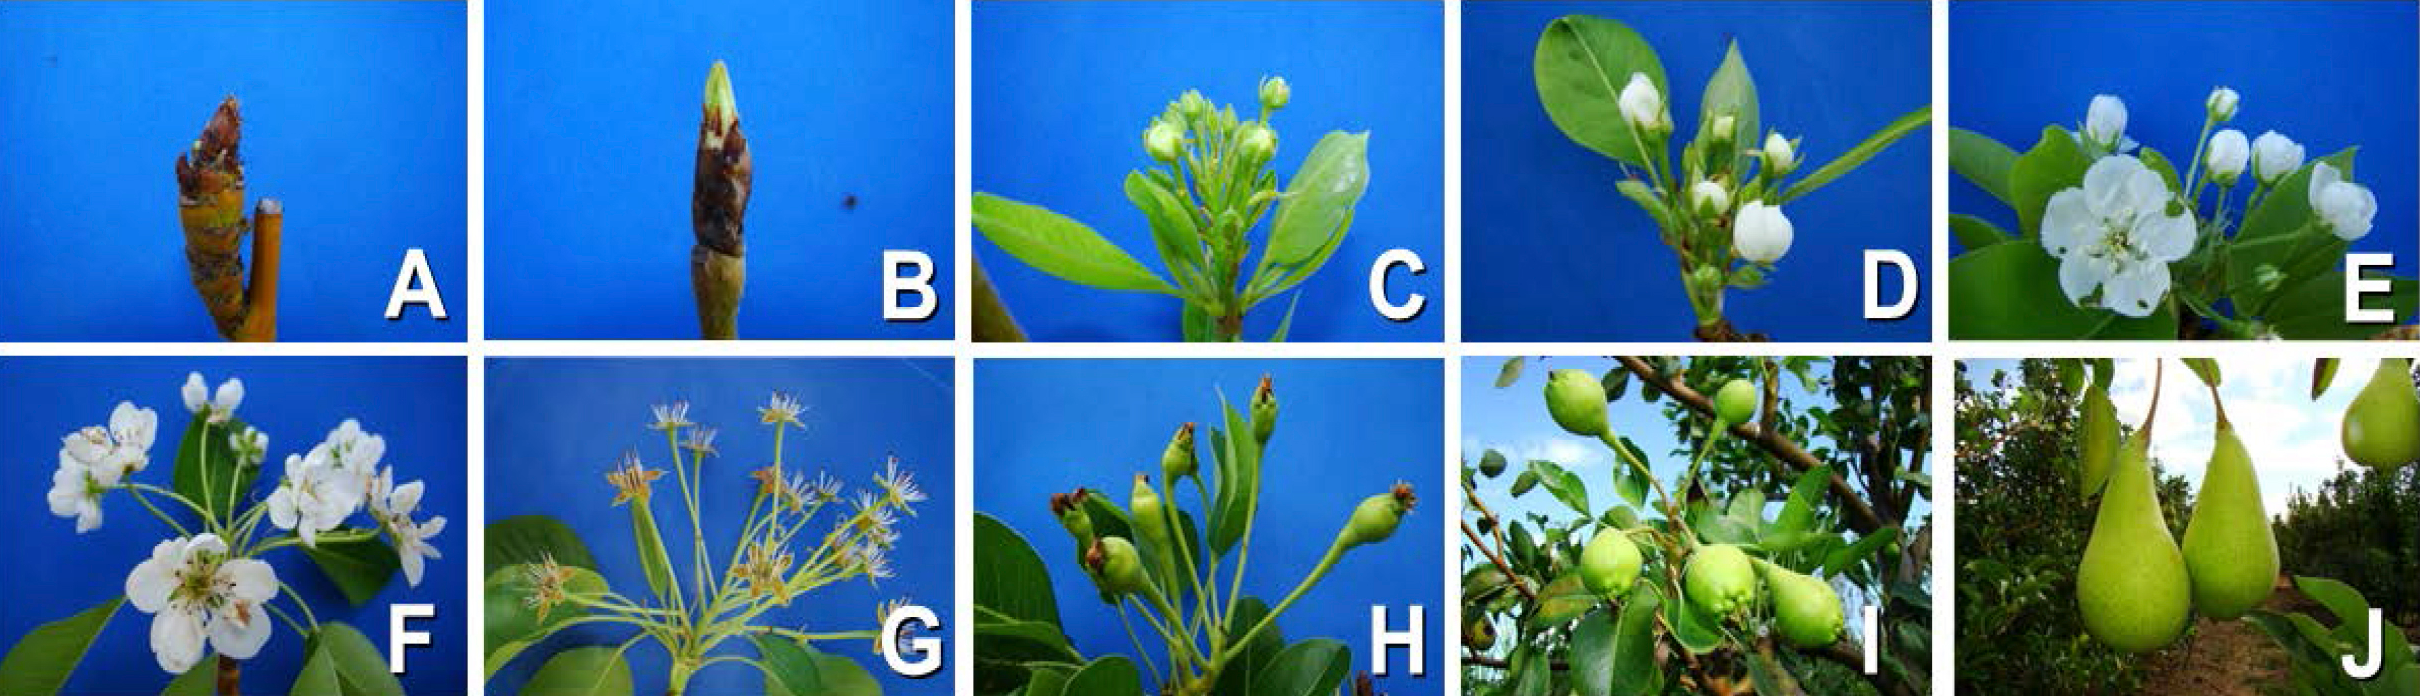
\includegraphics[width=1\linewidth]{pheno_pear_raw}
  \caption{Phenological Stages of Pyrus Communis - by TheJentschLab \cite{TheJentschLab}}
  \label{fig:pheno_pear_raw}
\end{figure}


\subsection{Enemies}
\label{sec:problem_spreadsheets_enemies}

As mentioned in \ref{sec:digital_mapping_framework}, farming fields have, by default, ideal conditions for the development of life. This attracts new species to the farming field, which usually directly impacts the economic viability of the yield. They can compromise the appearance of the product which affects the final consumer and, therefore, translates into a cut on the income of the farming company.

Enemies can be of three major types:
\begin{description}
	\item [Parasitic plants] Plants growing in non-desirable places that derive some or all of its nutritional requirement from another living plant (or from resources allocated to it)
	\item [Pests] Animal organisms that parasitise the plants.  Usually ectoparasites such as mites, insects, molluscs, vertebrates or any other life form that consumes plant tissue.
	\item [Diseases] Caused by pathogens (infectious organisms) and environmental conditions (physiological factors). Organisms that cause infectious disease can be fungi, bacteria, viruses etc.
\end{description}

Farmers register major occurrences of any of these three enemy types on the field-notebooks.

\subsection{Treatments and Control}
\label{sec:problem_spreadsheets_control}

Farmers deal with different enemies in different ways. 

\begin{description}
	\item [Herbicide] Herbicides, also commonly known as weedkillers, are chemical substances used to control unwanted plants. Non-selective herbicides kill all plant material with which they come into contact (mostly used for construction). Selective herbicide control specific weed species, while leaving the desired crop relatively unharmed.
	\item [Pesticide] Used to control animal organism life forms.
	\begin{description}
		\item [Insecticide] Insecticides are substances used to kill insects. They include ovicides and larvicides used against insect eggs and larvae, respectively.
		\item [Acaricide] For acari pests. Acari (or Acarina) are a taxon of arachnids that contains mites and ticks.
	\end{description}
	\item [Fungicide] Active substance(chemical compound) or biological organism used to kill or inhibit fungi or fungal spores (diseases).
\end{description}

\section{Pests}
\label{sec:problem_pests}

From the Fitoagro project, it was possible to sample the most harmful pests to the Royal Gala Apple and the Pear "Rocha"  Tree species.

\begin{itemize}
	\item \textit{Dasineura pyri (Bouché)} - Pear leaf-curling midge
	\item \textit{Aphanostigma pyri} - Pear phylloxera, Pear bark aphid
	\item \textit{Cydia pomonella} - Codling moth
	\item \textit{Quadraspidiotus perniciosus} - San José scale, Pernicious scale, California scale
\end{itemize}

This section \ref{sec:problem_pests} is heavily based on the Pest Encyclopedia Hyppz. Hypzz is an encyclopaedic database of 297 records describing important pests (insects, mites, rodents, nematodes, gastropods and small vertebrates) in Western Europe.

\subsection{Dasineura pyri (Bouché)}
\label{sec:problem_pests_cecidomia}

\begin{figure}[htbp]
  \centering
  \subcaptionbox{\textit{Dasineura pyri} adult drawn from a microscope setting.\label{fig:dasineura}}%
    {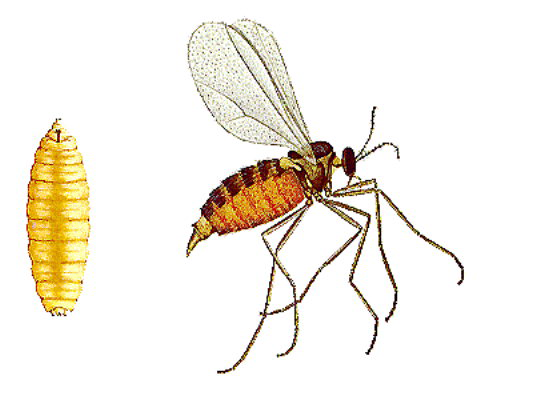
\includegraphics[width=0.55\linewidth]{dasineura}}%
  \hfill  
  \subcaptionbox{Damage on \textit{} The terminal leaves are severely distorted (arrowed).\label{fig:pear_rocha}}%
    {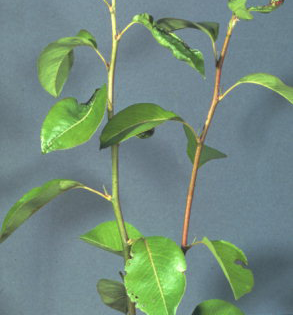
\includegraphics[width=0.42\linewidth]{dasineura_effects}}%
  \caption{\textit{Dasineura pyri} and its effects on \textit{Pyrus Communis}}
  \label{fig:dasineura_figs}
\end{figure}

Dasineura is a genus of midges in the family Cecidomyiidae. 

\subsubsection{Description}

\begin{description}
	\item [Adult] 2 to 3 mm. Black. In the female, the ovipositor is able to extend considerably (up to body length).
	\item [Eggs] Reddish.
	\item [Larva] 2 mm. Tapered at each end, pronounced tranverse segmentation, well-developed sternal spatula. Yellowish-white.
\end{description}

\subsubsection{Biology}

\begin{description}
	\item [Host plant] Pear
	\item [Adult] Very short life.
	\item [Fecundity] 30 eggs.
	\item [Eggs] Time until hatching, 3 to 4 days.
	\item [Larva] Time until pupation: 10 to 12 days
\end{description}

\subsubsection{Life Cycle}

3 to 6 generations per year. The adults appear in the spring, mate and lay eggs the same day. The female deposits the eggs on the underside of the still-furled leaf edges. The larva discharges saliva containing an auxin-related toxic substance over the leaves enabling it to feed on the cell contents. Some of the larvae pupate within the curled-up leaf, others fall to the ground, bury themselves and undergo diapause in a cocoon. Pupation begins in March.

\subsubsection{Damage}

The young leaves of attacked shoots remain curled up longitudinally. The leaf blade thickens considerably, becoming rigid and brittle. The 2nd and 3rd generations cause the greatest damage since they occur when shoot vigour and the formation of young leaves is most prolific.

\subsubsection{Monitoring}

\begin{figure}[htbp]
  \centering
  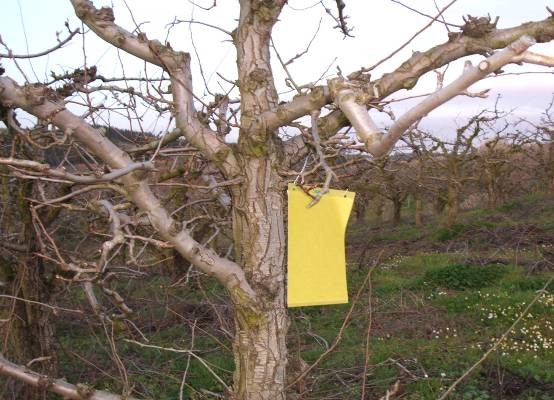
\includegraphics[width=0.7\linewidth]{dasineura_monitoring}
  \caption{Chromotropic trap made of adhesive sheet}
  \label{fig:dasineura_monitoring}
\end{figure}

Risk estimation for the Dasineura pyri pest is calculated based on the visual observation of damages on fruits, by sampling 100 sprouts in 50 trees from April to June. The economic level of attack is 15\% for saplings (young trees) and 50\% for adult trees.

Biological observations should monitor five sprouts (apples or pears) in 20 trees spread across the field. Observations should happen weekly between sprouting and late July.

Adult captures are usually performed with chromotropic traps as seen in figure \ref{fig:dasineura_monitoring}.  The chromotropic traps are adhesive sheets made of stiff and resistant plastic, with its two sides covered by a high-quality dry glue, water resistant, with no toxic substances and high-temperatures resistant.

\subsection{Aphanostigma pyri - Pear phylloxera}
\label{sec:problem_pests_filoxera}

\begin{figure}[htbp]
  \centering
  \subcaptionbox{\textit{Aphanostigma pyri} specimen.\label{fig:aphanostigma}}%
    {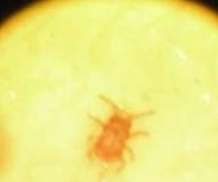
\includegraphics[width=0.45\linewidth]{aphanostigma}}%
  \hfill
  \subcaptionbox{Colony in the spring. Females, eggs and young nymphs.\label{fig:aphanostigma_effects}}%
    {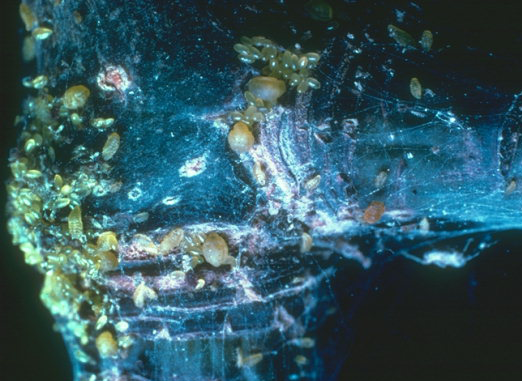
\includegraphics[width=0.5\linewidth]{aphanostigma_effects}}%
  \caption{\textit{Aphanostigma pyri} specimen and colony}
  \label{fig:dasineura_figs}
\end{figure}

\subsubsection{Description}

The insect is a holocyclic phylloxerid with the following biological phases:
\begin{itemize}
	\item Virginiparae and sexuparous females of piriform shape, whitish or lemon yellow with a length of 0.8-1.0 mm with well developed piercing-sucking mouthparts.
	\item Smaller (about 0.5 mm) sexuales with no mouthparts, ovoid in form.
	\item Eggs of sexuparae of a yellow green colour.
	\item Winter eggs with a diameter of 0.3 mm.
\end{itemize}

\subsubsection{Biology}

 The host is pear. Most attacked cultivars are, in Portugal, Passe Crassane, Comice, Douillard and Rocha. Other varieties are also attacked but less seriously.

\subsubsection{Life Cycle}

The complete life-cycle is as follows: virginiparous females hatch from winter eggs giving rise to several generations of identical types of female. Sexuparae appear in September. These lay male and female eggs from which, in the autumn, the sexuales emerge. After mating these lay the winter eggs.

In Portugal it is not known if the complete life-cycle, as described, occurs every year. No winter eggs have been found in certain areas. The overwintering form being then the parthenogenetic female.

\subsubsection{Damage}
In August sexuparae take shelter in the apical growth especially on those of late varieties where this area does not close completely. The feeding activity of these females produces large black areas on the fruit.

These black areas will appear, sometimes on other parts of the fruit, for instance where a leaf or fruit touches another fruit. Occasionally the black lesions will occur in the peduncular groove.

The commercial value of the damaged fruits will be severely reduced, often by 50\% to 60\%. The damage may occur:
\begin{itemize}
	\item During the maturation period, on the tree.
	\item During the cold storage together with the lesions caused by storage rots.
\end{itemize}

\subsubsection{Monitoring}

\begin{figure}[htbp]
  \centering
  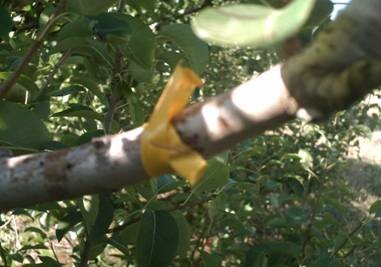
\includegraphics[width=0.7\linewidth]{aphanostigma_monitoring_1}
  \caption{WURTH Adhesive tape in a branch}
  \label{fig:aphanostigma_monitoring}
\end{figure}

\begin{figure}[htbp]
  \centering
  \subcaptionbox{\textit{Aphanostigma pyri} trap made of \textit{WURTH} adhesive tape.\label{fig:aphanostigma_monitoring_2}}%
    {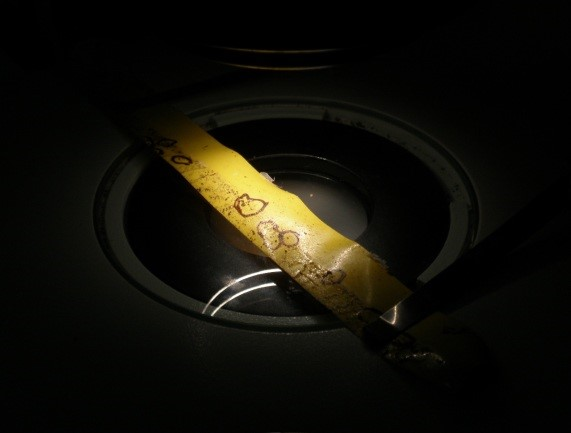
\includegraphics[width=0.47\linewidth]{aphanostigma_monitoring_2}}%
  \hfill
  \subcaptionbox{Trap under analysis in lab. \label{fig:aphanostigma_monitoring_3}}%
    {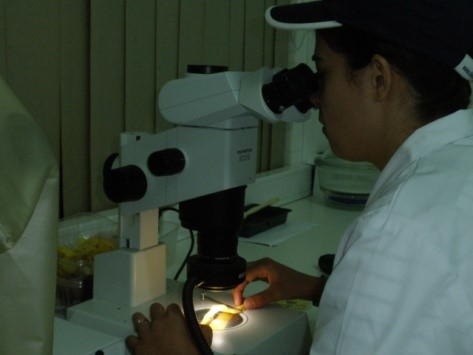
\includegraphics[width=0.47\linewidth]{aphanostigma_monitoring_3}}%
  \caption{\textit{Aphanostigma pyri} trap being analised in laboratory.}
  \label{fig:cydia_figs}
\end{figure}

Since different life cycles have been found, biological observations should provide risk estimations but, also answer some questions on how exactly how the species behaves, requirement for the FitoAgro project.

\begin{itemize}
	\item First appearance of the virginiparous females
	\item Migration to the fruit
	\item Descent from the fruit to the tree trunk
\end{itemize}

These moments above present key changes in the life cycle of this species, so they will be tracked by registering the presence of specimens in the tree trunk, branches, twigs and fruit.

The observation method is, to the say the least, interestic. WURTH Adhesive tape is used along with flannel patches, vaseline and plastic sheets. 

\begin{enumerate}
	\item Adhesive tape on trunk and two branches (opposing directions)
	\item Adhesive tape on four twigs with fruit.
	\item Fruit monitoring before harvest. Three fruits from random trees, plus three fruits from trees that were tracked during that season.
	\item Fruit monitoring during harvest - Five fruits from each of ten random trees, plus five fruits from each of ten tree that were tracked during that season. Cut fruit through the middle to test presence of specimens.
	\item Flannel patches after harvesting until next season. By april, apply vaseline on the flannel patches.
\end{enumerate}


\subsection{Cydia Pomonella - Codling moth}

\begin{figure}[htbp]
  \centering
  \subcaptionbox{\textit{Cydia Pomonella} adult.\label{fig:cydia}}%
    {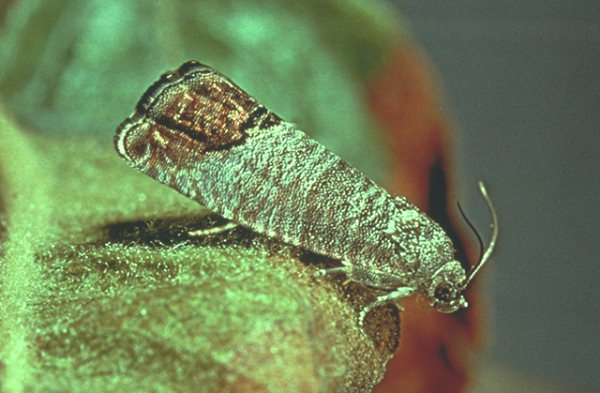
\includegraphics[width=0.5\linewidth]{cydia}}%
  \hfill
  \subcaptionbox{Second instar larva. Devouring the pips in the carpellary cavity.\label{fig:cydia_effects}}%
    {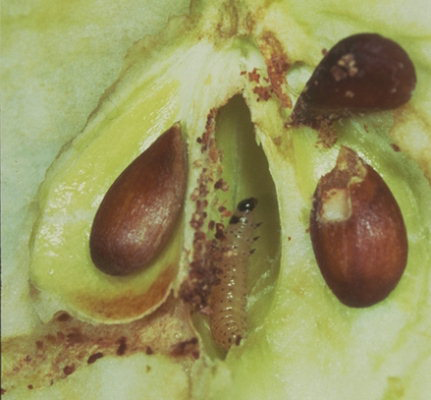
\includegraphics[width=0.4\linewidth]{cydia_effects}}%
  \caption{\textit{Cydia pomonella} adult and larva phases.}
  \label{fig:cydia_figs}
\end{figure}

\subsubsection{Description}

\begin{description}
	\item [Adult] Wingspan 16 to 19 mm. Very obvious and characteristic brown oval marking, surrounded by 2 shiny golden brown lines, tending towards the bronze, on the grey fore wings. Hind wings reddish brown, delicately ciliated.
	\item [Eggs] 1 mm diameter. Circular, flattened, slightly swollen in the middle. Laid singly on the upper side of the leaf, on the fruit or twig. Milky-white at first, then, a few days later, with presence of a reddish ring at the periphery.
	\item [Larva] 16 to 20 mm. Head dark brown; body pale pink to reddish. Abdominal prolegs, anal prolegs.
	\item [Pupa] 10 to 12 mm. Yellow-brown to dark brown. Occuring in silky cocoon.
\end{description}

\subsubsection{Biology}

\begin{description}
	\item [Host plants] Apricot, quince, walnut, pear, apple and sometimes peach and plum.
	\item [Adult] Medium longevity, 15 to 18 days. Active during the day at temperatures of > 15°C.
	\item [Fecundity] 30 to 50 eggs, on average.
	\item [Eggs] Time until hatching, 18 days at 15°C, and 6 at 25°C.
	\item [Larva] Developmental duration, 20 to 30 days.
	\item [Pupa] Developmental duration, 20 to 28 days.
\end{description}

\subsubsection{Life Cycle}

The eggs hatch at the end of May. The caterpillar first undergoes a so-called "wandering stage" (2 to 5 days). After a couple of exploratory bites, it penetrates a fruit where a second fruit or a leaf is touching, or at the stalk or stalk-eye. When development is completed, it leaves the fruit and weaves a cocoon in a sheltered spot. From then onwards, two developmental routes are possible: it will either pupate and give rise to a 2nd-generation of moth, or enter diapause. The caterpillars that become fully fed from August to October all enter diapause. They overwinter in cocoons hidden in cracks in the tree-trunk or in a natural shelter on the soil.

Pupation in April. The adults emerge at the end of April, beginning of May. They mate and lay the eggs on leaves, twigs, or young fruits.

\subsubsection{Damage}

On pomaceous fruit, around the entrance hole made by the young larva, a gnawed area, followed by a spiral gallery leading down to the pips which the caterpillar also eats. On walnuts, the caterpillar burrows through the husk to the kernel; when the latter hardens, it leaves by the hilum or remains in the husk. The bite marks on the damaged fruit makes them impossible to sell. Damaged fruit drops prematurely.
Late or seasonal varieties of pear are not very susceptible to the 1st generation because their epidermis is hard.

\subsubsection{Monitoring}

Biological observations should monitor fifty fruits per tree on a total of twenty trees spread randomly across the farming field. Observations should occur once per week. 

Risk estimation for the Cydia pomonella pest is calculated based on the visual observation of damages on fruits. The attack percentage is the percentage of attacked fruits in a total sample of one thousand fruits. 

Capturing is achieved by releasing sexual pheromones inside a trap as seen in figure \ref{fig:cydia_monitoring}. Number of caught specimens should be recorded, the trap cleaned and set up for the next week.


\begin{figure}[htbp]
  \centering
  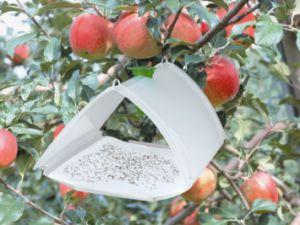
\includegraphics[width=0.7\linewidth]{cydia_monitoring}
  \caption{Sexual pheromone trap for \textit{Cydia Pomonella}}
  \label{fig:cydia_monitoring}
\end{figure}

\subsection{Quadraspidiotus perniciosus}

\begin{figure}[htbp]
  \centering
  \subcaptionbox{\textit{Quadraspidiotus perniciosus} male and female individuals. The scale of the female was turned upside down to show the colour of the body of the female. Young nymphs can be seen (arrowed).\label{fig:quadraspidiotus}}%
    {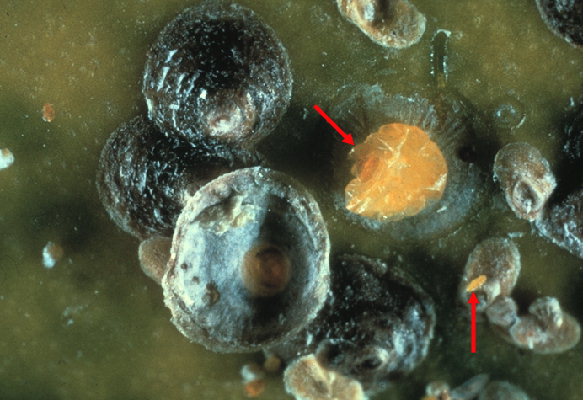
\includegraphics[width=0.47\linewidth]{quadraspidiotus}}%
  \hfill
  \subcaptionbox{Damage on pear. The change in colour of the epidermis is due to the presence of scale insects. Figure from Hyppz \cite{AlainFraval} \label{fig:quadraspidiotus_effects}}%
    {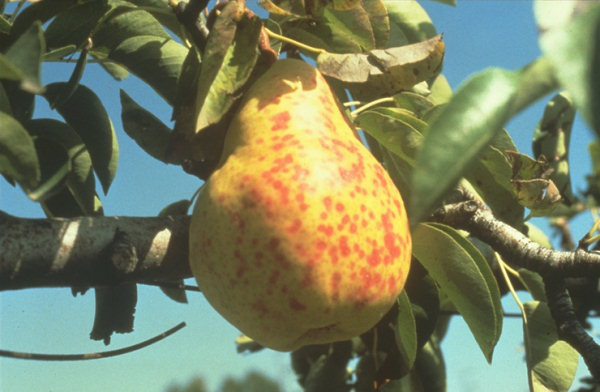
\includegraphics[width=0.47\linewidth]{quadraspidiotus_effects}}%
  \caption{\textit{Quadraspidiotus perniciosus} male, female and effects on product.}
  \label{fig:quadraspidiotus_figs}
\end{figure}

\subsubsection{Description}

\begin{description}
	\item [Adult] Female apterous, pear-shaped, flattened, fixed to the plant and hidden under a detachable scale. Scale circular, dark grey, about 2 mm across. Males provided with a pair of wings.
	\item [Nymph] Young nymph mobile, yellow, provided with 3 pairs of short legs. Once fixed, secretes a white scale which becomes grey and finally black.
\end{description}

\subsubsection{Biology}

Also know as Cochonilha, \textit{Quadraspidiotus perniciosus} is very polyphagous and develops on more than 150 species of host, especially on apple, pear, plum, peach, cherry, currant, black currant.

Nymphs overwinter during the 1st instar in a state of diapause. After moulting twice (in March and May), they emerge either as males or females. Females are viviparous and each produces 8-10 nymphs per day from late May onwards, the egg-laying period spreading over 6 weeks. The average number of nymphs produced on a favorable host plant is 400.

Nymphs are at first mobile and then settle down by inserting their stylets into plant cells. They produce encrustations on twigs, branches and sometimes on leaves and fruits.

\subsubsection{Life Cycle}

There are 2-4 generations depending on the region. As soon as winter approaches, first generation nymphs enter a state of diapause. Very young and second-generation nymphs as well as adults, die.

\subsubsection{Damage}

Feed by these insects, when they inject toxic saliva, leads to a distortion of plant tissue, the premature dropping of leaves and the discoloration of the fruits' epidermis as well as the decline of affected twigs and branches.
A specific parasite of this pest, Prospaltella perniciosi, has been introduced in some studies to fight against this scale insect.

\subsubsection{Monitoring}

Risk estimation for the Quadraspidiotus perniciosus pest is calculated based on the visual observation of branches and twigs. Percentage of attacked fruits in a total sample of one hundred fruits is the attack percentage. 

Biological observations are performed with sticky pads (seen in figure \ref{fig:quadraspidiotus_monitoring}) and should monitor five twigs per tree on a total of twenty trees spread randomly across the farming field. Observations should occur once per week by registering whether the twigs show symptoms of the insect or not. After renewal of the traps, these are sent to laboratory for species determination and counting.


\begin{figure}[htbp]
  \centering
  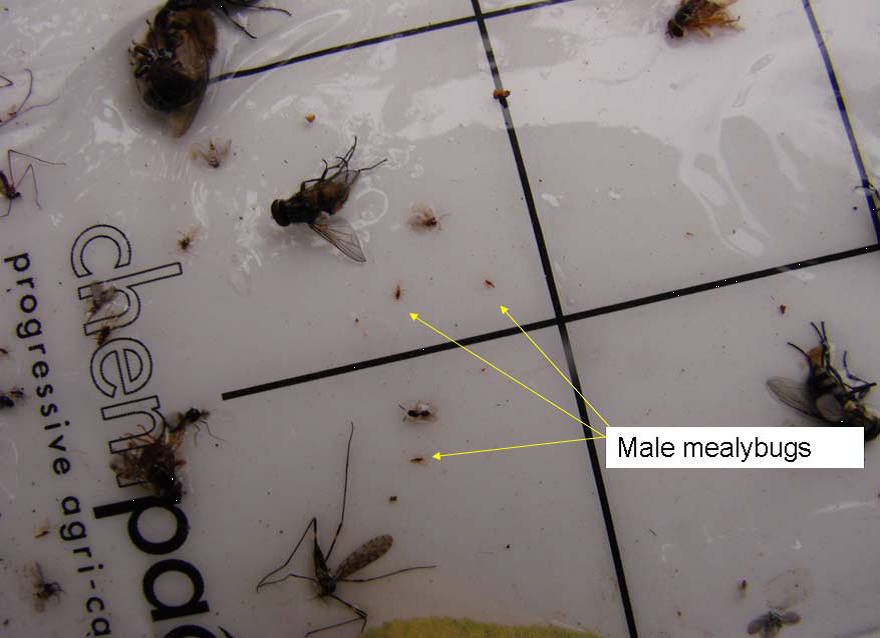
\includegraphics[width=0.7\linewidth]{quadraspidiotus_monitoring}
  \caption{Sampling of \textit{Quadraspidiotus perniciosus} males on a sticky pad.}
  \label{fig:quadraspidiotus_monitoring}
\end{figure}

\section{Data Collection}
\label{sec:problem_data_collection}

Most of the farmers and agronomists have worked in the very same fields their whole life so they know where specific events happen: the spots with less solar exposure, the irrigation defects and details, the places where water leaks, the spots with pest occurrences, the phenological cycles, the history of the field, etc. Mentally or using non-appropriate registering methodologies, they track the field variables without a proper tool.

As agricultural teams grow bigger, some information is registered to be consulted by all team members (or to keep an history). But even then, data is manually added to a spreadsheet, being Google drive the common sharing pattern among the "more advanced" cooperatives and farming companies (information from a FitoAgro project meeting).

Processing all this information requires precise and normalized inputs. This will be the main focus of this dissertation: Gathering the available data from the field to the server in an effortless and consistent way.

Even if out of the scope of this work, it is studied mostly in the state of the art, how it would be possible to fully automate the biological counting and analysis of the known enemy species by crop. Since this presents a significant problem by itself (a device that counts and analysis automatically the pests per tree that needs low to no maintenance), pseudo-automated data-collection is the closest path to ideal data-collection. Pseudo-automated data collection meaning that humans will play a key role in the registering of occurrences but some extra processing should be done in the background to ease out the task for the user.
